\subsection{Sixth Experience}

\subsubsection{Python TCP Server-Client Implementation}
For this experience we needed to capture on the loopback (lo) interface of wireshark, because we are going to send a file to our own machine.

\begin{figure}[htbp]
	\centering
	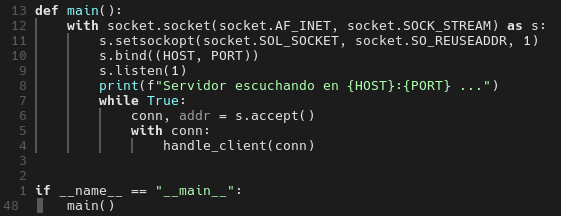
\includegraphics[width=1\linewidth]{img/sixth_experience/1.png}
	\caption{}\label{fig:4_1}
\end{figure}

\begin{figure}[htbp]
	\centering
	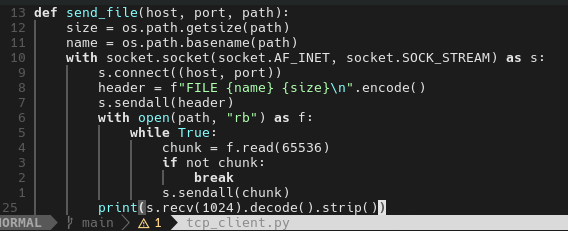
\includegraphics[width=1\linewidth]{img/sixth_experience/2.png}
	\caption{}\label{fig:4_1}
\end{figure}

For this purpose we set the port and host with the bind function of the library socket of Python. To ensure the three-way handshake we used the connect function on the client, and the listen and accept functions on the server, all functions of the same library.

\begin{figure}[htbp]
	\centering
	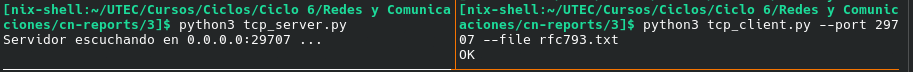
\includegraphics[width=1\linewidth]{img/sixth_experience/3.png}
	\caption{}\label{fig:4_1}
\end{figure}

Finally, we open two terminals on the same computer and in one we runned the tcp\_server.py file and in the other one the tcp\_client.py file with the corresponding host, port and a file to test the connection and, as we can see in the figure above, it connected with no problem.

\subsubsection{Sending a file}

Well, we already have sended a file for testing the TCP connection.

\begin{figure}[htbp]
	\centering
	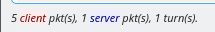
\includegraphics[width=1\linewidth]{img/sixth_experience/4.png}
	\caption{}\label{fig:4_1}
\end{figure}

\begin{figure}[htbp]
	\centering
	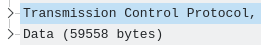
\includegraphics[width=1\linewidth]{img/sixth_experience/5.png}
	\caption{}\label{fig:4_1}
\end{figure}

We can see in the figures above that just 5 packages were transmitted, because the packet size of my computer is really big, about 60000 bytes.
There where no retransmissions because the communication is local. Both the secuence and acknowledgment numbers increase accordingly to the amount of bytes that have been already transmitted. If the size of the file was larger, there would have been more packages, but this wasn't the case.

